\subsubsection{React Context}

В типичном React приложении данные передаются сверху вниз от родительского компоненту к дочернему с помощью пропсов~\cite{react}. Однако при сложной логике приложения, например, когда необходимо передавать одни и те же данные нескольким компонентам (например, выбранная тема оформления страниц или язык), такой подход будет неэффективен.

Для решения этой проблемы можно воспользоваться следующими решениями:

\begin{enumerate}
  \item Redux (менеджер состояний).
  \item React Context.
\end{enumerate}

Библиотека Redux является наиболее популярным менеджером состояний~\cite{redux}. С помощью этой библиотеки можно управлять состоянием и потоками данных всего приложения. Данные в Redux представляются единым объектом состояния -- state. Напрямую данные в state изменять нельзя, необходимо использование действий -- action и редукторов -- reducer~\cite{redux}. При этом action представляет из себя объект, описывающий какие именно изменения необходимо произвести, для передачи этого объекта от приложения хранилищу необходим вызов функции dispatch, содержащий тип изменения и данные на изменение. Reducer в сою очередь является функцией, получающее действие и в соответствии с этим действием изменяет состояние хранилища. На рисунке~\ref{img:react__redux} представлена общая схема взаимодействия элементов Redux. View здесь является компонентом React.

\begin{figure}[H]
  \centering
  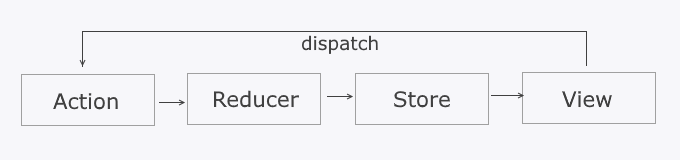
\includegraphics[width=0.9\textwidth]{assets/images/theoretical2/redux.png}
  \caption{Общая схема взаимодействия элементов Redux}
  \label{img:react__redux}
\end{figure}

Использование Redux необходимо, когда невозможно эффективно управлять состоянием, используя лишь возможности React. Так как для небольших приложений можно передавать данные во все необходимые компоненты без потерь в эффективности и увеличения сложности логики приложения, применение Redux необходимо лишь для более сложных приложений.

В простых приложениях более предпочтительно использование React Con\-text (контекст), предоставляемого библиотекой React. С помощью контекста можно обеспечить доступ к данным во многих компонентах на разных уровнях вложенности, не передавая их на каждом уровне вложенности~\cite{react}.

Для передачи данных вниз по дереву используется компонент Provider. Любой компонент, являющийся дочерним к этому, имеет доступ к этим данным, вне зависимости от глубины вложенности.

Для создания контекста используется функция createContext. При этом создаётся объект Context. Когда React отображает компонент, подписанный на этот объект, React получает значение в контексте из ближайшего подходящего Provider в дереве компонентов~\cite{react}.

Компонент Provider принимает проп value, который будет передан во все дочерние компоненты, использующие этот контекст. При изменении переданных данных в контексте все компоненты, использующие этот контекст, будут заново отображаться на странице.

Для подписки на изменения контекста используется компонент Consumer. Этот компонент принимает функцию в качестве дочернего компонента, которая принимает текущее значение контекста и возвращает React компонент.

Также для подписки на изменения контекста можно воспользоваться хуком useContext, который возвращает текущее значение контекста.

На рисунке~\ref{img:react__context} представлен пример использования React Context. В компоненте App применяется контекст ThemeContext, предоставляющий дочерним компонентам светлую и тёмную тему оформления. Компонент ThemeButton получит текущее значение темы без прямой передачи ему этого значения через пропсы.

\begin{figure}[H]
  \centering
  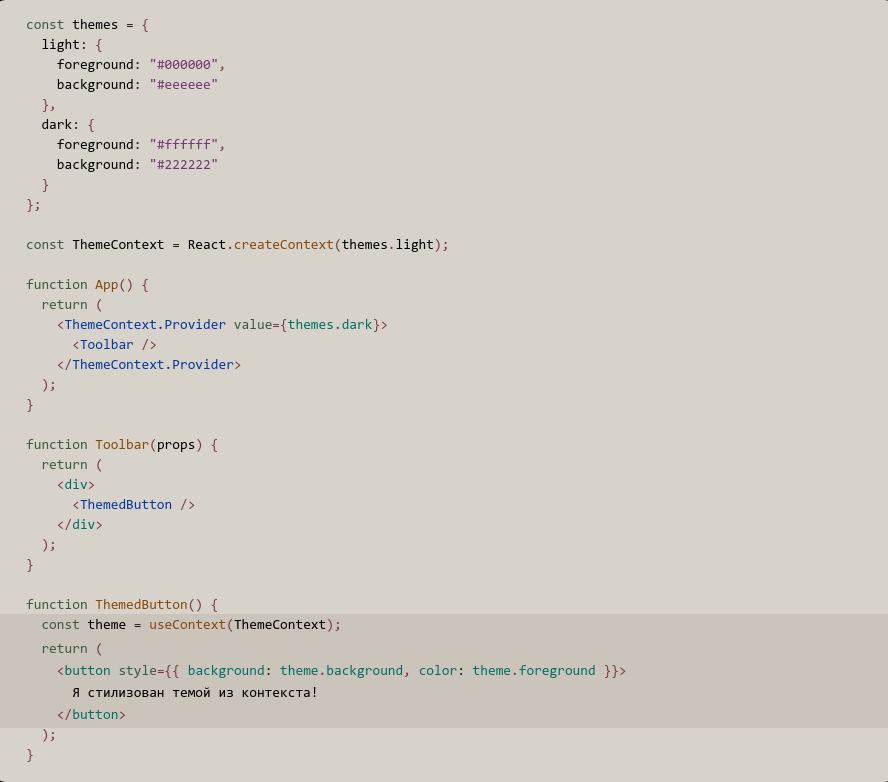
\includegraphics[height=0.4\textheight]{assets/images/theoretical2/react_context.png}
  \caption{Пример использования React Context}
  \label{img:react__context}
\end{figure}

Результат отображения компонента App при использовании светлой темы представлен на рисунке~\ref{img:react__context-light}, тёмной темы -- на рисунке~\ref{img:react__context-dark}.

\begin{figure}[H]
  \centering
  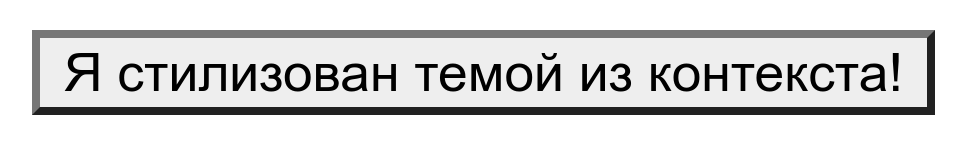
\includegraphics[width=0.9\textwidth]{assets/images/theoretical2/react_context-light.png}
  \caption{Отображение светлой темы}
  \label{img:react__context-light}
\end{figure}

\begin{figure}[H]
  \centering
  
\includegraphics[width=0.9\textwidth]{assets/images/theoretical2/react_context-dark.png}
  \caption{Отображение тёмной темы}
  \label{img:react__context-dark}
\end{figure}